\section{Test 1: Radial Spokes from the Origin and Length--Weight Duality}
\label{sec:vectors}

In the fabrication suite \texttt{magicGemWeb} \cite{mathewson2025magicgemweb}, the $16$ cells of an order-four magic square are built as two radial sculptures pivoted at the origin $O$: (i)~a \emph{3D $16$-spoke hub-and-strut star} (\texttt{magicGem.scad}, \Cref{fig:origin-vectors-3d}(a)) with spokes $\mathbf p_{ij}(\lambda)=(x_j,y_i,\lambda z_{ij})$ of length $R_{ij}(\lambda)=\|\mathbf p_{ij}(\lambda)\|_2$ along unit directions $\hat{\mathbf p}_{ij}(\lambda)=\mathbf p_{ij}(\lambda)/R_{ij}(\lambda)\in S^2$; and (ii)~a \emph{planar $16$-spoke balance wheel} on a conical fulcrum (\texttt{weighted\_ring.stl}, \Cref{fig:ring-vectors}(a)) with spokes along $\mathbf r_{ij}=(x_j,y_i)$ of radius $r_{ij}=\|\mathbf r_{ij}\|_2$ and unit direction $\mathbf u_{ij}=\mathbf r_{ij}/r_{ij}\in S^1$. At natural linear lengths ($L_{ij}=R_{ij}(\lambda)$ or $\ell(r_{ij})=r_{ij}$), both sculptures balance identically at $O$ because $\sum_{i,j}\mathbf p_{ij}(\lambda)=\mathbf 0$ and $\sum_{i,j}z_{ij}\mathbf r_{ij}=\mathbf 0$ \cite{loly2004invariance,rogers2005multipole}, closing the $16$ planar vectors into a head-to-tail polygon (\Cref{fig:ring-vectors}(b)).

Our first test probes the mechanism of this equilibrium: \emph{does radial balance reside in the directions of the spokes alone, or does it rely on the unequal spoke lengths compensating the unequal directions? When equalizing spoke lengths breaks balance, how can an opposing inequality in tip weights or power-law lengths restore it?}

\subsection{Length--Weight Duality: Why Equalizing Spoke Lengths Breaks Balance}

\begin{definition}[Generalized 3D and planar origin-vector resultants]
\label{def:radial-resultant}
For an arrangement $S$ of order $n$ and vertical lift scale $\lambda>0$, let $R_{ij}(\lambda)=\sqrt{x_j^2+y_i^2+\lambda^2z_{ij}^2}$ and $\hat{\mathbf p}_{ij}(\lambda)=\mathbf p_{ij}(\lambda)/R_{ij}(\lambda)$ ($\mathbf 0$ if $R_{ij}(\lambda)=0$). Given cell weights $w=(w_{ij})$ and prescribed 3D spoke lengths $L=(L_{ij})$, the \emph{3D origin-vector resultant} is
\begin{equation}
\label{eq:V-3d-general}
\mathbf V_{w,L}(S;\lambda) = \sum_{i,j} w_{ij}\,L_{ij}\,\hat{\mathbf p}_{ij}(\lambda)
= \sum_{R_{ij}(\lambda)>0} \left(\frac{w_{ij}L_{ij}}{R_{ij}(\lambda)}\right)\mathbf p_{ij}(\lambda) \in \R^3.
\end{equation}
For equal weights $w_{ij}=1$ and power-law 3D lengths $L_{ij}=R_{ij}(\lambda)^\beta$ ($\beta\in\R$), we write
\begin{equation}
\label{eq:V-beta}
\mathbf V_\beta(S;\lambda) := \sum_{i,j} R_{ij}(\lambda)^\beta\,\hat{\mathbf p}_{ij}(\lambda)
= \sum_{i,j} R_{ij}(\lambda)^{\beta-1}\,\mathbf p_{ij}(\lambda) \in \R^3,
\end{equation}
and for weighted unit vectors ($L_{ij}=1$) on $S^2$, we write $\mathbf B^{(3)}_{w,\lambda}(S):=\mathbf V_{w,1}(S;\lambda)=\sum_{i,j}w_{ij}\hat{\mathbf p}_{ij}(\lambda)$. Similarly, in the grid plane, given cell masses $m=(m_{ij})$ and a radial length profile $\ell\colon[0,\infty)\to[0,\infty)$ along unit rays $\mathbf u_{ij}=\mathbf r_{ij}/r_{ij}$, the \emph{planar radial resultant} is
\begin{equation}
\label{eq:B-planar}
\mathbf B_{m,\ell}(S) = \sum_{i,j} m_{ij}\,\ell(r_{ij})\,\mathbf u_{ij}
= \sum_{r_{ij}>0} \left(\frac{m_{ij}\ell(r_{ij})}{r_{ij}}\right)(x_j,y_i) \in \R^2.
\end{equation}
\end{definition}

Because $\ell(r_{ij})$ depends only on the radius $r_{ij}$, grid symmetry gives $\sum_{i,j}\ell(r_{ij})\mathbf u_{ij}=\mathbf 0$, so replacing the positive entry masses $m_{ij}=s_{ij}=\bar s+z_{ij}$ by the signed heights $m_{ij}=z_{ij}$ leaves the planar resultant unchanged: $\mathbf B_{s,\ell}(S)=\mathbf B_{z,\ell}(S)$.

\begin{proposition}[Length--weight duality and the order-three two-ring warm-up]
\label{prop:reciprocity}
Let $n\ge3$ and $\lambda>0$.
\begin{enumerate}
\item \emph{(3D and 2D length--weight duality.)} Scaling 3D vector lengths from the origin to $L_{ij}$ with weights $w_{ij}$ produces the same resultant \eqref{eq:V-3d-general} as keeping the natural 3D vectors $\mathbf p_{ij}(\lambda)$ ($L'_{ij}=R_{ij}(\lambda)$) and assigning effective weights $w'_{ij}=w_{ij}L_{ij}/R_{ij}(\lambda)$. In particular:
\begin{enumerate}
\item Power-law 3D vector lengths $L_{ij}=R_{ij}(\lambda)^\beta$ with unit weights ($w_{ij}=1$) are mechanically dual to natural 3D vectors $\mathbf p_{ij}(\lambda)$ with weights $w'_{ij}=R_{ij}(\lambda)^{\beta-1}$.
\item Unit-length 3D vectors on $S^2$ ($L_{ij}=1$) balance identically ($\sum_{i,j}w_{ij}\hat{\mathbf p}_{ij}(\lambda)=\mathbf 0$) for every arrangement $S$ if weighted by their unequal 3D lengths $w_{ij}=c\,R_{ij}(\lambda)$ ($c\in\R$).
\item In the grid plane, unit vectors $\mathbf u_{ij}$ balance for every semi-magic square ($\sum_{i,j}m_{ij}\mathbf u_{ij}=\mathbf 0$) whenever $m_{ij}=c\,z_{ij}r_{ij}$, and a radial profile $\ell_{ij}$ with $m_{ij}=z_{ij}$ balances every semi-magic square if and only if $(\ell_{ij}/r_{ij})\mathbf r_{ij}$ has components in the row--column subspace $W_{\mathrm{rc}}=\{a(x_j)+b(y_i)\}$.
\end{enumerate}
\item \emph{(Order-three exact formula.)} At order $n=3$, the eight non-central cells of $A_3$ lie on two concentric rings: four edge midpoints $R_1=\{(\pm1,0),(0,\pm1)\}$ ($r_1=1$) and four corners $R_{\sqrt{2}}=\{(\pm1,\pm1)\}$ ($r_2=\sqrt{2}$). Every semi-magic square $S$ of order~$3$ satisfies $\mathbf d_1(S)+\mathbf d_2(S)=\mathbf 0$, where $\mathbf d_k(S)=\sum_{(i,j)\in R_k}z_{ij}\mathbf r_{ij}$, and hence
\begin{equation}
\label{eq:n3-radial}
\mathbf B_{z,\ell}(S) = \left(\ell(1) - \frac{\ell(\sqrt{2})}{\sqrt{2}}\right)\mathbf d_1(S).
\end{equation}
For all eight magic squares of order~$3$ (the $D_4$-orbit of the Lo Shu square), $\|\mathbf d_1(S)\|_2=\sqrt{80}=4\sqrt{5}$, giving
\begin{equation}
\label{eq:n3-norm}
\|\mathbf B_{z,\ell}(S)\|_2 = 4\sqrt{5}\,\left|\ell(1) - \frac{\ell(\sqrt{2})}{\sqrt{2}}\right|,
\qquad
\|\mathbf B_{\mathrm{unit}}(S)\|_2 = 4\sqrt{5} - 2\sqrt{10} \approx 2.619717.
\end{equation}
Thus $\mathbf B_{z,\ell}(S)=\mathbf 0$ at $n=3$ if and only if $\ell(\sqrt{2})=\sqrt{2}\,\ell(1)$.
\end{enumerate}
\end{proposition}

\begin{proof}
Part~(1) follows directly from \eqref{eq:V-3d-general}--\eqref{eq:B-planar}, the identity $\sum_{i,j}\mathbf p_{ij}(\lambda)=\mathbf 0$, and the characterization of $W_{\mathrm{rc}}$ as the orthogonal complement of the zero-line-sum space \cite[Sect.~2]{mathewson2026moments}. In Part~(2), $\mathbf r_{11}=(0,0)$ implies $\mathbf d_1(S)+\mathbf d_2(S)=\sum_{i,j}z_{ij}\mathbf r_{ij}=\mathbf 0$ for every semi-magic square, which yields \eqref{eq:n3-radial} upon grouping \eqref{eq:B-planar} over $R_1$ and $R_{\sqrt{2}}$. Evaluating $\mathbf d_1=(-8,4)$ on the Lo Shu square gives $\|\mathbf d_1\|_2=\sqrt{80}=4\sqrt{5}$, and $D_4$-invariance of the Euclidean norm yields \eqref{eq:n3-norm}.
\end{proof}

\Cref{prop:reciprocity} makes the mechanics of spoke normalization transparent: forcing unequal spokes to equal unit length ($L_{ij}=1$ or $\ell=1$) divides each coordinate vector by its irrational radius $R_{ij}(\lambda)$ or $r_{ij}$. At order $n=3$, the corner ring sits at an irrational ratio $r_2/r_1=\sqrt{2}$, so equalizing the spoke lengths breaks the cancellation between $\mathbf d_1$ and $\mathbf d_2=-\mathbf d_1$. We now see how this irrationality mechanism operates across the three concentric rings of order $n=4$.

\subsection{Planar Balance Wheels: The \texorpdfstring{$\sqrt{5}$}{sqrt(5)} Irrationality Barrier and Power-Law Restoration}

At order $n=4$, the sixteen cells of $A_4=\{-\frac32,-\frac12,\frac12,\frac32\}^2$ partition into three concentric rings around the origin $O$ (\Cref{fig:hero-squares}(b), \Cref{fig:ring-vectors}(a)):
\begin{align*}
R_{\mathrm{in}} &= \bigl\{(\pm\tfrac12,\pm\tfrac12)\bigr\} && (4\text{ inner cells},\quad r_1 = \tfrac{\sqrt{2}}{2}),\\
R_{\mathrm{mid}} &= \bigl\{(\pm\tfrac32,\pm\tfrac12),\,(\pm\tfrac12,\pm\tfrac32)\bigr\} && (8\text{ edge-interior cells},\quad r_2 = \tfrac{\sqrt{10}}{2}),\\
R_{\mathrm{out}} &= \bigl\{(\pm\tfrac32,\pm\tfrac32)\bigr\} && (4\text{ corner cells},\quad r_3 = \tfrac{3\sqrt{2}}{2}).
\end{align*}
Whereas the outer and inner radii have a rational ratio $r_3/r_1=3$, the middle and inner radii have the irrational ratio $r_2/r_1=\sqrt{5}\notin\Q$. Consequently, when spokes are trimmed to unit length ($\alpha=0$), the inner and outer rings combine into a rational lattice vector $\mathbf u(S)$ that attempts to cancel an irrational multiple $\mathbf v(S)/\sqrt{5}$ from the middle ring.

\begin{figure}[htbp]
\centering
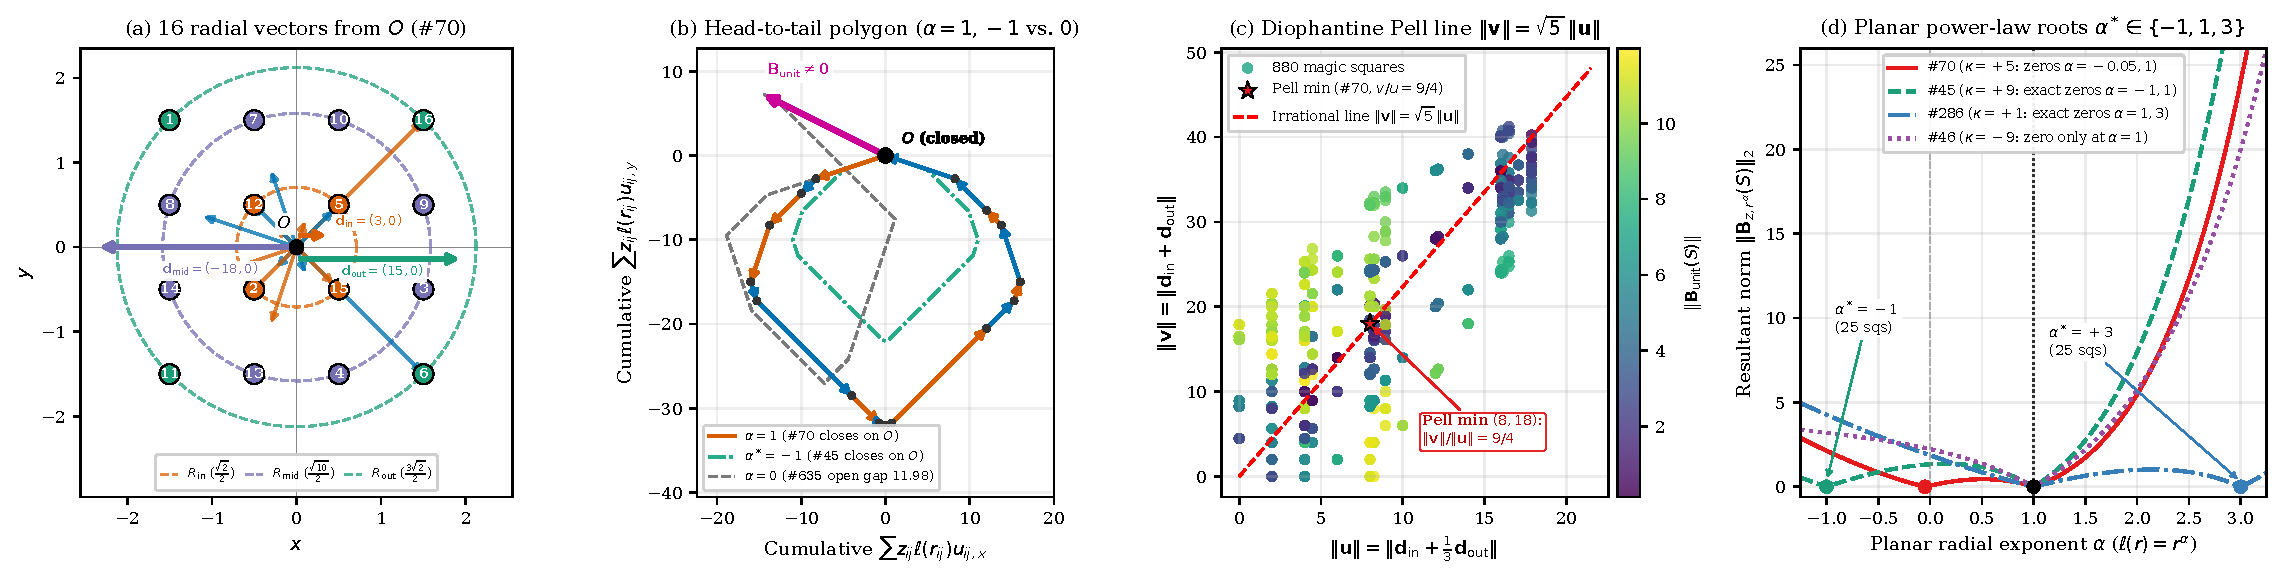
\includegraphics[width=\textwidth]{figures/fig_ring_vectors.pdf}
\caption{Planar radial vectors from the origin $O=(0,0)$, head-to-tail polygon closure, and the Diophantine Pell minimum at order four. (a)~The $16$ radial vectors $z_{ij}\mathbf r_{ij}$ radiating from $O$ (orange $z_{ij}>0$ outward, blue $z_{ij}<0$ inward) across the three concentric rings $R_{\mathrm{in}},R_{\mathrm{mid}},R_{\mathrm{out}}$ on square \#70, together with the three ring dipole resultants $\mathbf d_{\mathrm{in}}=(3,0)$, $\mathbf d_{\mathrm{out}}=(15,0)$, and $\mathbf d_{\mathrm{mid}}=(-18,0)$. (b)~Placing the $16$ vectors $z_{ij}\ell(r_{ij})\mathbf u_{ij}$ head-to-tail in order of angle around $O$ produces a closed $16$-gon at linear lengths $\alpha=1$ ($\ell(r)=r$ on \#70, solid orange/blue) and at inverse radial lengths $\alpha^*=-1$ ($\ell(r)=1/r$ on \#45, green dash-dot), whereas unit lengths $\alpha=0$ ($\ell(r)=1$ on \#635, dashed) fail to close by the magenta gap vector $\mathbf B_{\mathrm{unit}}(S)$. (c)~Scatter plot of $\|\mathbf v(S)\|_2=\|\mathbf d_{\mathrm{in}}+\mathbf d_{\mathrm{out}}\|_2$ versus $\|\mathbf u(S)\|_2=\|\mathbf d_{\mathrm{in}}+\frac13\mathbf d_{\mathrm{out}}\|_2$ across all $880$ magic squares against the irrational balance line $\|\mathbf v\|=\sqrt{5}\,\|\mathbf u\|$, with the eight Pell-minimum squares ($v/u=9/4$) marked by red stars. (d)~Resultant norm $\|\mathbf B_{z,r^\alpha}(S)\|_2$ versus power-law exponent $\alpha$, highlighting the universal root at $\alpha=1$ and the exact second roots at $\alpha^*=-1$ (\#45, $\kappa=+9$), $\alpha^*=-0.050$ (\#70, $\kappa=+5$), and $\alpha^*=+3$ (\#286, $\kappa=+1$).}
\label{fig:ring-vectors}
\end{figure}

\begin{theorem}[Three-Ring Decomposition, Irrationality No-Go, and Pell Minimum]
\label{thm:three-ring}
For any arrangement $S$ of order $4$, define the three ring dipole vectors radiating from $O$:
\[
\mathbf d_{\mathrm{in}}(S) = \sum_{c\in R_{\mathrm{in}}} z_c\mathbf r_c,\qquad
\mathbf d_{\mathrm{mid}}(S) = \sum_{c\in R_{\mathrm{mid}}} z_c\mathbf r_c,\qquad
\mathbf d_{\mathrm{out}}(S) = \sum_{c\in R_{\mathrm{out}}} z_c\mathbf r_c.
\]
\begin{enumerate}
\item \emph{(Ring sums, integrality, and non-vanishing.)} For every $4\times4$ arrangement $S$ of distinct integers, $\mathbf d_{\mathrm{in}}(S)\ne\mathbf 0$ and $\mathbf d_{\mathrm{out}}(S)\ne\mathbf 0$. For every order-four magic square $S\in\mathcal M_4$, both $R_{\mathrm{in}}$ and $R_{\mathrm{out}}$ sum to $\mu_4=34$ (so $\sum_{c\in R_{\mathrm{in}}}z_c=\sum_{c\in R_{\mathrm{out}}}z_c=0$), and hence $\mathbf d_{\mathrm{in}}(S)\in\Z^2\setminus\{\mathbf 0\}$ and $\mathbf d_{\mathrm{out}}(S)\in(3\Z)^2\setminus\{\mathbf 0\}$, with
\begin{equation}
\label{eq:ring-lower}
\|\mathbf d_{\mathrm{in}}(S)\|_2 \ge 1,\qquad \|\mathbf d_{\mathrm{out}}(S)\|_2 \ge 3.
\end{equation}
\item \emph{(Three-ring formula.)} Whenever $\sum_{c\in A_4}z_c\mathbf r_c=\mathbf 0$ (in particular, for every semi-magic square), $\mathbf d_{\mathrm{mid}}(S)=-\bigl(\mathbf d_{\mathrm{in}}(S)+\mathbf d_{\mathrm{out}}(S)\bigr)$, and for every radial length profile $\ell=(\ell_1,\ell_2,\ell_3)$ on $(r_1,r_2,r_3)$,
\begin{equation}
\label{eq:three-ring-general}
\mathbf B_{z,\ell}(S) = \left(\frac{\ell_1}{r_1} - \frac{\ell_2}{r_2}\right)\mathbf d_{\mathrm{in}}(S)
+ \left(\frac{\ell_3}{r_3} - \frac{\ell_2}{r_2}\right)\mathbf d_{\mathrm{out}}(S).
\end{equation}
\item \emph{(No-go theorem for unit vectors and even power laws.)} For planar unit vectors ($\ell_1=\ell_2=\ell_3=1$, i.e.\ $\alpha=0$), substituting $1/r_1=\sqrt{2}$, $1/r_3=\sqrt{2}/3$, and $1/r_2=\sqrt{2}/\sqrt{5}$ into \eqref{eq:three-ring-general} separates the rational $\sqrt{2}$ coefficients from the irrational $\sqrt{2}/\sqrt{5}$ coefficient:
\begin{equation}
\label{eq:unit-uv}
\mathbf B_{\mathrm{unit}}(S) = \sqrt{2}\,\left(\mathbf u(S) - \frac{1}{\sqrt{5}}\,\mathbf v(S)\right),
\end{equation}
where $\mathbf u(S)=\mathbf d_{\mathrm{in}}(S)+\frac13\mathbf d_{\mathrm{out}}(S)\in\Z^2$ collects the inner and outer ring contributions and $\mathbf v(S)=\mathbf d_{\mathrm{in}}(S)+\mathbf d_{\mathrm{out}}(S)=-\mathbf d_{\mathrm{mid}}(S)\in\Z^2$ is the negative middle-ring dipole. Because $\sqrt{5}\notin\Q$ and $\mathbf d_{\mathrm{in}}(S),\mathbf d_{\mathrm{out}}(S)\ne\mathbf 0$, \emph{no $4\times4$ arrangement of distinct integers with vanishing first moments (and hence no $4\times4$ semi-magic or magic square) ever satisfies $\mathbf B_{\mathrm{unit}}(S)=\mathbf 0$}, nor can $\mathbf B_{z,r^\alpha}(S)=\mathbf 0$ hold for any even integer $\alpha\in2\Z$.
\item \emph{(Exact Diophantine Pell minimum over $\mathcal M_4$.)} Across all $880$ magic squares of order~$4$, the global minimum of $\|\mathbf B_{\mathrm{unit}}(S)\|_2$ is
\begin{equation}
\label{eq:pell-min}
\min_{S\in\mathcal M_4} \|\mathbf B_{\mathrm{unit}}(S)\|_2
= \frac{18\sqrt{10}}{5} - 8\sqrt{2}
= \frac{2\sqrt{10}}{5(9+4\sqrt{5})}
= \frac{2\sqrt{10}}{5\varphi^6} \approx 0.07049108,
\end{equation}
where $\varphi=(1+\sqrt{5})/2$. This minimum is attained when $\mathbf d_{\mathrm{out}}(S)=5\mathbf d_{\mathrm{in}}(S)$ with $\|\mathbf d_{\mathrm{in}}(S)\|_2=3$, where $\mathbf u(S)$ and $\mathbf v(S)$ are parallel in the ratio $\|\mathbf v\|/\|\mathbf u\|=18/8=9/4$, the fundamental Pell convergent to $\sqrt{5}$ ($9^2-5\cdot4^2=1$). Up to $D_4$-symmetry, exactly eight magic squares achieve \eqref{eq:pell-min}: squares \#70, \#76, \#121, \#188, \#452, \#459, \#490, and \#574, all in Dudeney's Group~VI.
\end{enumerate}
\end{theorem}

\begin{proof}
(1) Labelling the four entries of $R_{\mathrm{in}}$ at $(-\frac12,\frac12)$, $(\frac12,\frac12)$, $(-\frac12,-\frac12)$, $(\frac12,-\frac12)$ by $a,b,c,d\in\Z$ gives $\mathbf d_{\mathrm{in}}(S)=\frac12\bigl((b+d)-(a+c),(a+b)-(c+d)\bigr)$. If $\mathbf d_{\mathrm{in}}(S)=\mathbf 0$, then $b+d=a+c$ and $a+b=c+d$; adding and subtracting these equations forces $b=c$ and $a=d$, contradicting that $S$ has distinct entries. For $S\in\mathcal M_4$, subtracting the sum of all $16$ cells ($4\mu_4$) from the sum of the two outer rows and two outer columns ($R_0+R_3+C_0+C_3=4\mu_4$) gives $\sum_{c\in R_{\mathrm{out}}}s_c-\sum_{c\in R_{\mathrm{in}}}s_c=0$, while the two main diagonals sum to $D_1+D_2=\sum_{c\in R_{\mathrm{out}}}s_c+\sum_{c\in R_{\mathrm{in}}}s_c=2\mu_4$; hence $\sum_{c\in R_{\mathrm{in}}}s_c=\sum_{c\in R_{\mathrm{out}}}s_c=\mu_4=34$ (an even integer), which implies $\mathbf d_{\mathrm{in}}(S)\in\Z^2\setminus\{\mathbf 0\}$. Since the corner coordinates are $(\pm\frac32,\pm\frac32)=3(\pm\frac12,\pm\frac12)$, identical algebra gives $\mathbf d_{\mathrm{out}}(S)\in(3\Z)^2\setminus\{\mathbf 0\}$ and \eqref{eq:ring-lower}.

(2) Partitioning $A_4=R_{\mathrm{in}}\sqcup R_{\mathrm{mid}}\sqcup R_{\mathrm{out}}$ gives $\mathbf d_{\mathrm{mid}}=-(\mathbf d_{\mathrm{in}}+\mathbf d_{\mathrm{out}})$, and substituting this relation into \eqref{eq:B-planar} yields \eqref{eq:three-ring-general}.

(3) Setting $\ell_1=\ell_2=\ell_3=1$ with $1/r_1=\sqrt{2}$, $1/r_2=\sqrt{2}/\sqrt{5}$, and $1/r_3=\sqrt{2}/3$ in \eqref{eq:three-ring-general} gives $\mathbf B_{\mathrm{unit}}(S)=(\sqrt{2}-\sqrt{2}/\sqrt{5})\mathbf d_{\mathrm{in}}+(\sqrt{2}/3-\sqrt{2}/\sqrt{5})\mathbf d_{\mathrm{out}}=\sqrt{2}\bigl((\mathbf d_{\mathrm{in}}+\frac13\mathbf d_{\mathrm{out}})-\frac{1}{\sqrt{5}}(\mathbf d_{\mathrm{in}}+\mathbf d_{\mathrm{out}})\bigr)$, which is \eqref{eq:unit-uv}. Because $\mathbf u(S),\mathbf v(S)\in\Z^2$ by~(1) and $\sqrt{5}\notin\Q$, $\mathbf B_{\mathrm{unit}}(S)=\mathbf 0$ requires $\mathbf u(S)=\mathbf v(S)=\mathbf 0$, which forces $\mathbf d_{\mathrm{in}}(S)=\mathbf d_{\mathrm{out}}(S)=\mathbf 0$, contradicting~(1). The same irrationality holds for any even exponent $\alpha=2m$, where $r_2^{\alpha-1}/r_1^{\alpha-1}=5^{m-1}\sqrt{5}\notin\Q$.

(4) Since $\mathbf v(S)-\mathbf u(S)=\frac23\mathbf d_{\mathrm{out}}(S)\in(2\Z)^2$, the integer vectors satisfy the parity congruence $\mathbf u(S)\equiv\mathbf v(S)\pmod 2$ for every semi-magic square, while $\mathbf d_{\mathrm{in}},\mathbf d_{\mathrm{out}}\ne\mathbf 0$ implies $\mathbf u\ne\mathbf v$ and $\mathbf v\ne 3\mathbf u$. Decomposing $\mathbf v$ parallel and orthogonal to $\mathbf u$ shows that $\|\mathbf u-\mathbf v/\sqrt{5}\|_2$ is minimized when $\mathbf u=p\mathbf e$ and $\mathbf v=q\mathbf e$ are collinear along a primitive lattice direction $\mathbf e=(a,b)\in\Z^2$ ($\gcd(a,b)=1$), where $\|\mathbf B_{\mathrm{unit}}(S)\|_2=\sqrt{2(a^2+b^2)}\,|p-q/\sqrt{5}|$ and the prefactor $\sqrt{2(a^2+b^2)}$ is minimal along the coordinate axes ($a^2+b^2=1$). Over all integer pairs with $p\equiv q\pmod 2$, the best approximations to $\sqrt{5}$ are governed by the Pell--Lucas equation $q^2-5p^2=\pm 4$, whose positive solutions $(p,q)=(F_k,L_k)$ alternate between odd--odd Fibonacci--Lucas semiconvergents such as $(3,7)$, $(5,11)$, $(13,29)$, $(21,47)$ ($k\not\equiv 0\pmod 3$) and even--even pairs $(F_{3m},L_{3m})=2(p_m,q_m)$ obtained by doubling the principal continued-fraction convergents $q_m/p_m\in\{2/1,9/4,38/17,\dots\}$ of $\sqrt{5}=[2;\overline{4}]$. On $\mathcal M_4$, every pair $(F_k,L_k)$ with $k\ge 7$ is excluded on two independent grounds:
\begin{enumerate}
\item[(i)] \emph{Direct axial collinear bound:} Since $\frac13\mathbf d_{\mathrm{out}}=\frac12(\mathbf v-\mathbf u)$ and $\mathbf d_{\mathrm{in}}=\frac12(3\mathbf u-\mathbf v)$, realizing $(p,q)=(F_k,L_k)$ along a coordinate axis requires $\frac13|d_{\mathrm{out}}|=\frac12(L_k-F_k)$. Across $\mathcal M_4$, $\frac13\|\mathbf d_{\mathrm{out}}\|_\infty\le 12$, which immediately excludes all $k\ge 8$ ($\frac12(L_k-F_k)\ge\frac12(47-21)=13>12$). For $k=7$, $(F_7,L_7)=(13,29)$ requires $\frac13|d_{\mathrm{out}}|=\frac12(29-13)=8$ and $|d_{\mathrm{in}}|=\frac12(39-29)=5$; however, saturating $\frac13|d_{\mathrm{out}}|=8$ along a coordinate axis on $\mathcal M_4$ constrains the inner-ring dipole on every axial collinear square ($\mathbf d_{\mathrm{in}}\parallel\mathbf d_{\mathrm{out}}$) to $|d_{\mathrm{in}}|\le 4$ and hence $p=|d_{\mathrm{in}}+\frac13d_{\mathrm{out}}|\le 12<13$.
\item[(ii)] \emph{Even-lattice property:} Subtracting $C_1+C_2=2\mu_4$ and $C_0+C_3=2\mu_4$ from $D_1+D_2=2\mu_4$ gives $s_{00}+s_{03}=s_{31}+s_{32}$ and $s_{11}+s_{12}=s_{20}+s_{23}$, and across all $24$ modulo-$2$ parity patterns of $\mathcal M_4$ the four top diagonal cells $T_{\mathrm{diag}}=\{(0,0),(0,3),(1,1),(1,2)\}$ (and likewise $R_{\mathrm{diag}}=\{(0,3),(3,3),(1,2),(2,2)\}$) always have an even sum $\sum_{c\in T_{\mathrm{diag}}}s_c\in\{18,20,\dots,42\}$. Because $u_y(S)=\sum_{c\in T_{\mathrm{diag}}}s_c-34$ and $u_x(S)=\sum_{c\in R_{\mathrm{diag}}}s_c-34$, every magic square $S\in\mathcal M_4$ satisfies
\[
\mathbf u(S) = 2\tilde{\mathbf u}(S) \in (2\Z)^2,\enspace
\mathbf v(S) = 2\tilde{\mathbf v}(S) \in (2\Z)^2,\enspace
\|\mathbf u(S)\|_\infty \le 16,\enspace
\|\mathbf u(S)\|_2 \le 8\sqrt{5} \approx 17.89,
\]
excluding all odd--odd Pell--Lucas pairs and reducing \eqref{eq:unit-uv} to $\|\mathbf B_{\mathrm{unit}}(S)\|_2=2\sqrt{2}\,\|\tilde{\mathbf u}(S)-\tilde{\mathbf v}(S)/\sqrt{5}\|_2$ with $\tilde{\mathbf u}(S),\tilde{\mathbf v}(S)\in\Z^2$ and $\|\tilde{\mathbf u}(S)\|_2\le 4\sqrt{5}<9$.
\end{enumerate}
By Lagrange's theorem on continued fractions, across all integer denominators $1\le\tilde u<17$, the unique best rational approximation to $\sqrt{5}$ is the fundamental Pell convergent $\tilde v/\tilde u=9/4$ ($9^2-5\cdot 4^2=1$), corresponding to $(p,q)=(F_6,L_6)=(8,18)$ and giving $2\sqrt{2}(9/\sqrt{5}-4)=18\sqrt{10}/5-8\sqrt{2}=2\sqrt{10}/(5\varphi^6)\approx0.07049108$ (since $\varphi^6=(2+\sqrt{5})^2=9+4\sqrt{5}$), whereas the next convergent $38/17$ requires $\|\tilde{\mathbf u}\|_2\ge 17>4\sqrt{5}$. On square \#70 (\Cref{fig:hero-squares}(b)), the inner ring $\{5,12,2,15\}$ gives $\mathbf d_{\mathrm{in}}=\frac12\bigl((12+15)-(5+2),(12+5)-(2+15)\bigr)=(3,0)$ and the outer corners $\{1,16,11,6\}$ give $\mathbf d_{\mathrm{out}}=\frac32\bigl((16+6)-(1+11),(1+16)-(11+6)\bigr)=(15,0)=5\mathbf d_{\mathrm{in}}$, realizing $\mathbf u=(8,0)$, $\mathbf v=(18,0)$, and \eqref{eq:pell-min}.
\end{proof}

How, then, can a planar balance wheel achieve exact equilibrium at a non-linear length profile $\ell(r)=r^\alpha$ ($\alpha\ne1$)? Equation~\eqref{eq:three-ring-general} shows that balance is restored whenever the inner and outer ring dipoles align in the same direction ($\mathbf d_{\mathrm{out}}=\kappa\mathbf d_{\mathrm{in}}$ with $\kappa>0$), so that both rings jointly oppose the middle ring $\mathbf d_{\mathrm{mid}}=-(1+\kappa)\mathbf d_{\mathrm{in}}$ (\Cref{fig:ring-vectors}(d)).

\begin{corollary}[Restoring planar balance via power-law exponents $\alpha^*\ne1$]
\label{cor:planar-power-roots}
For power-law radial lengths $\ell(r)=r^\alpha$ ($\alpha\in\R$), equation~\eqref{eq:three-ring-general} takes the form
\begin{equation}
\label{eq:planar-power-form}
\mathbf B_{z,r^\alpha}(S) = r_1^{\alpha-1}\Bigl[\bigl(1 - 5^{(\alpha-1)/2}\bigr)\mathbf d_{\mathrm{in}}(S) + \bigl(3^{\alpha-1} - 5^{(\alpha-1)/2}\bigr)\mathbf d_{\mathrm{out}}(S)\Bigr].
\end{equation}
\begin{enumerate}
\item Because $1<\sqrt{5}<3$, the ratio $h(\alpha)=\frac{5^{(\alpha-1)/2}-1}{3^{\alpha-1}-5^{(\alpha-1)/2}}$ (extended by $h(1)=\frac{\ln 5}{\ln(9/5)}\approx2.7381$) is a strictly decreasing bijection from $\R$ onto $(0,\infty)$. Consequently, an order-four magic square $S$ possesses a second power-law balance exponent $\alpha^*(S)\ne1$ satisfying $\mathbf B_{z,r^{\alpha^*}}(S)=\mathbf 0$ if and only if $\mathbf d_{\mathrm{in}}(S)$ and $\mathbf d_{\mathrm{out}}(S)$ are strictly parallel ($\mathbf d_{\mathrm{out}}(S)=\kappa\mathbf d_{\mathrm{in}}(S)$ with $\kappa>0$), which holds for $204$ of the $880$ magic squares (while $204$ squares have anti-parallel dipoles $\kappa<0$).
\item Across all $880$ magic squares, the second root $\alpha^*(\kappa)$ is an integer in only two cases:
\begin{itemize}
\item $\alpha^*=-1$ (inverse radial lengths $\ell(r)=1/r$), corresponding to $\kappa=h(-1)=+9$, achieved by $25$ squares (e.g.\ square \#45 in \Cref{fig:hero-squares}(c), where $\mathbf d_{\mathrm{in}}=(0,-2)$ and $\mathbf d_{\mathrm{out}}=(0,-18)=9\mathbf d_{\mathrm{in}}$);
\item $\alpha^*=+3$ (cubic radial lengths $\ell(r)=r^3$), corresponding to $\kappa=h(3)=+1$, achieved by $25$ squares (e.g.\ square \#286).
\end{itemize}
For the $17$ squares with $\kappa=+5$ (including the eight Pell-minimum squares of \Cref{thm:three-ring}(4)), the exact zero occurs at $\alpha^*(5)\approx -0.0496$, explaining why $\|\mathbf B_{z,r^\alpha}(S)\|_2$ pinches nearly to zero at $\alpha=0$ (\Cref{fig:ring-vectors}(d)).
\end{enumerate}
\end{corollary}

\begin{proof}
Setting \eqref{eq:planar-power-form} to $\mathbf 0$ for $\alpha\ne1$ requires $\mathbf d_{\mathrm{out}}(S)=h(\alpha)\mathbf d_{\mathrm{in}}(S)$. Since $1<5^{t/2}<3^t$ for $t=\alpha-1>0$ and $3^t<5^{t/2}<1$ for $t<0$, both numerator and denominator of $h(\alpha)$ have the sign of $\alpha-1$, so $h(\alpha)>0$ with $\lim_{\alpha\to-\infty}h(\alpha)=+\infty$ and $\lim_{\alpha\to+\infty}h(\alpha)=0$. Since $\kappa\in\Q_{>0}$ cannot equal the transcendental number $\frac{\ln 5}{\ln(9/5)}$, every square with $\kappa>0$ has a unique root $\alpha^*(\kappa)=h^{-1}(\kappa)\ne1$. By \Cref{thm:three-ring}(3), an integer root $\alpha^*\ne1$ must be odd, $\alpha^*=2m+1$ ($m\in\Z\setminus\{0\}$), where $h(2m+1)=\frac{5^m-1}{9^m-5^m}$; comparing this sequence against the $15$ positive rational ratios $\kappa$ realized on $\mathcal M_4$ leaves only $m=-1$ ($\kappa=9$, $25$ squares) and $m=+1$ ($\kappa=1$, $25$ squares).
\end{proof}

\subsection{Three-Dimensional Spoke Stars: Unit-Sphere Counterweights and Cubic Vertical Balance}

We now lift the spoke sculpture into three dimensions (\Cref{fig:origin-vectors-3d}). In 3D, trimming all $16$ spokes to the unit sphere $S^2$ ($\beta=0$) breaks equilibrium on $832$ of the $880$ squares, sparing only the $48$ associative squares of Group~III where antipodal pairs cancel pairwise ($\hat{\mathbf p}_{-c}=-\hat{\mathbf p}_c$). Nevertheless, because the natural unequal lengths $R_{ij}(\lambda)>0$ satisfy $\sum_{i,j}R_{ij}(\lambda)\hat{\mathbf p}_{ij}(\lambda)=\mathbf 0$, the origin $O$ always lies strictly inside the convex hull of the $16$ unit rays, guaranteeing that positive unequal tip weights $\mathbf w^*>\mathbf 0$ restore unit-sphere equilibrium for every magic square.

\begin{figure}[htbp]
\centering
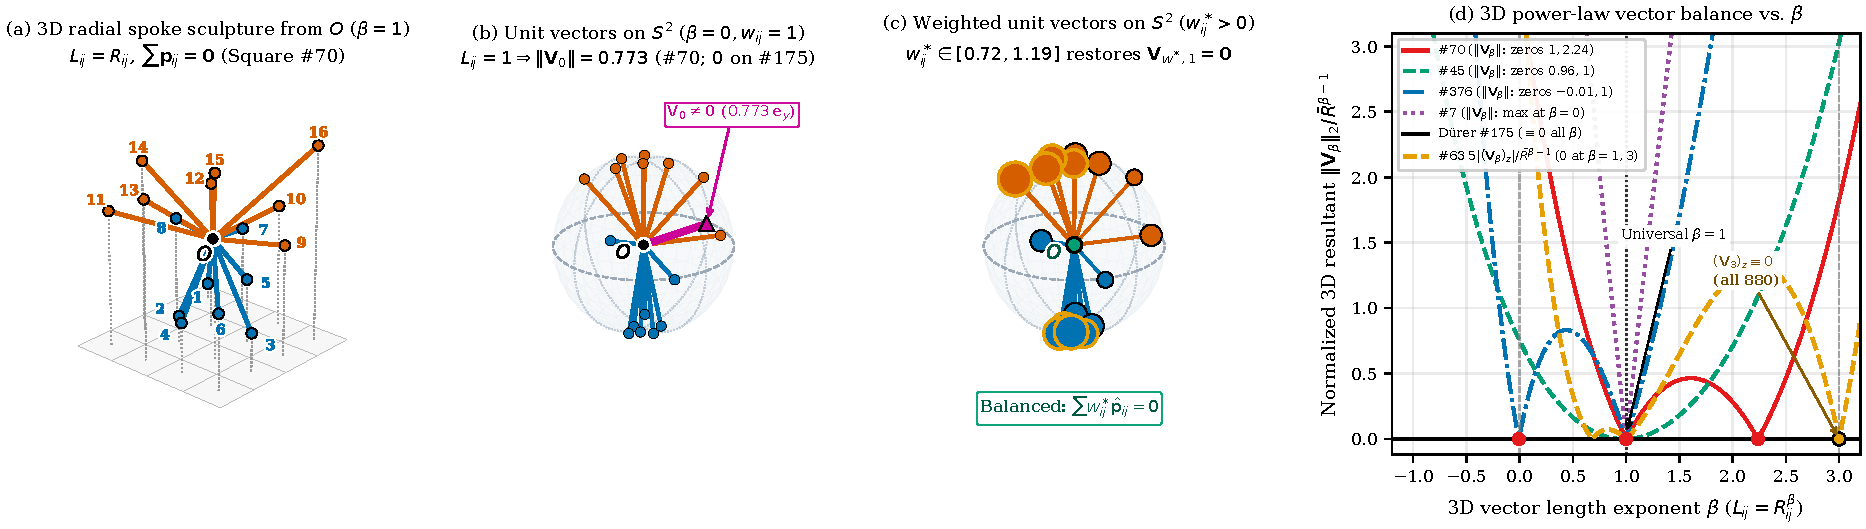
\includegraphics[width=\textwidth]{figures/fig_origin_vectors_3d.pdf}
\caption{Three-dimensional radial spoke sculptures from the origin $O=(0,0,0)$ of variable length and tip weight. (a)~The $16$-spoke radial sculpture $\mathbf p_{ij}$ ($\beta=1$, spoke length $L_{ij}=R_{ij}$, orange for $z_{ij}>0$, blue for $z_{ij}<0$) of non-associative square \#70 over the floor grid, balancing identically at the central hub $O$ ($\sum\mathbf p_{ij}=\mathbf 0$). (b)~Trimming all $16$ spokes to unit length $L_{ij}=1$ ($\beta=0$, equal tip weights $w_{ij}=1$) on the unit sphere $S^2$ leaves a non-zero resultant $\mathbf V_0=(0,0.773,0)$ (magenta arrow) on square \#70, whereas antipodal pairs cancel on associative D\"urer \#175. (c)~Assigning the minimum-variance positive tip weights $w_{ij}^*\in[0.72,1.19]$ (sphere tip sizes, gold-rimmed for $w_{ij}^*>1$) restores exact unit-sphere balance $\sum w_{ij}^*\hat{\mathbf p}_{ij}=\mathbf 0$ at $O$. (d)~Normalized 3D power-law resultant $\|\mathbf V_\beta(S;1)\|_2/\bar R^{\beta-1}$ versus length exponent $\beta$, showing universal balance at $\beta=1$, second power-law roots $\beta^*\ne1$ on Group~VI squares (\#70 at $\beta^*=2.24$, \#45 at $0.96$, \#376 at $-0.008$), and identical vertical vanishing $(\mathbf V_3)_z=0$ at $\beta=3$ (gold dashed curve showing $5|(\mathbf V_\beta)_z|/\bar R^{\beta-1}$ on square \#63).}
\label{fig:origin-vectors-3d}
\end{figure}

\begin{theorem}[3D Power-Law Vectors, Cubic Vertical Vanishing, and Positive Unit-Sphere Weights]
\label{thm:3d-power}
Let $S$ be a semi-magic square of order $n$ and let $\lambda>0$.
\begin{enumerate}
\item \emph{(Cubic 3D vector law $\beta=3$.)} For cubic 3D spoke lengths $L_{ij}=R_{ij}(\lambda)^3$ from the origin (dual by \Cref{prop:reciprocity}(1) to weighting $\mathbf p_{ij}(\lambda)$ by $w_{ij}=R_{ij}(\lambda)^2=r_{ij}^2+\lambda^2z_{ij}^2$), the vertical $z$-component vanishes identically for every semi-magic square of any order $n$ and every $\lambda>0$:
\begin{equation}
\label{eq:V3-exact}
\mathbf V_3(S;\lambda) = \sum_{i,j}\bigl(r_{ij}^2+\lambda^2z_{ij}^2\bigr)(x_j,y_i,\lambda z_{ij})
= \biggl(\lambda^2\sum_{i,j}z_{ij}^2 x_j,\;\; \lambda^2\sum_{i,j}z_{ij}^2 y_i,\;\; 0\biggr).
\end{equation}
At order $n=4$, $\mathbf V_3(S;\lambda)=\mathbf 0$ if and only if $S$ is one of the $48$ associative magic squares.
\item \emph{(Unit-sphere parity and Group~VI power-law roots.)} Under any even weight function $w_{ij}=f(|z_{ij}|)$, every associative square satisfies $\hat{\mathbf p}_{-c}(\lambda)=-\hat{\mathbf p}_c(\lambda)$ and hence $\mathbf V_\beta(S;\lambda)=\mathbf 0$ for all $\beta\in\R$ and $\lambda>0$. At $n=4$, $\mathbf V_0(S;\lambda)=\mathbf 0$ holds if and only if $S$ is one of the $48$ associative squares ($\|\mathbf V_0(S;1)\|_2\in[0.0072,2.4284]$ on the remaining $832$ squares). Among the $304$ Group~VI squares (where $C_2$ symmetry confines $\mathbf V_\beta(S;\lambda)$ to a single coordinate axis), $107$ squares possess a second 3D power-law balance exponent $\beta^*(S)\in[-3,4]\setminus\{1\}$ with $\mathbf V_{\beta^*}(S;1)=\mathbf 0$ (\Cref{fig:origin-vectors-3d}(d)).
\item \emph{(Universal positive minimum-variance balancing weights on $S^2$.)} Letting $\hat P(\lambda)\in\R^{N\times 3}$ have rows $\hat{\mathbf p}_{ij}(\lambda)^{\top}$, the unique weight vector $\mathbf w^*(S;\lambda)$ of minimum Euclidean distance $\|\mathbf w-\mathbf 1\|_2$ from uniform weights $\mathbf 1$ satisfying $\sum_{i,j}w_{ij}^*\hat{\mathbf p}_{ij}(\lambda)=\mathbf 0$ is
\begin{equation}
\label{eq:w-star}
\mathbf w^*(S;\lambda) = \mathbf 1 - \hat P(\lambda)\bigl(\hat P(\lambda)^{\top}\hat P(\lambda)\bigr)^{-1}\mathbf V_0(S;\lambda).
\end{equation}
Across all $880$ order-four magic squares at $\lambda=1$, $\lambda_{\mathrm{iso}}=1/\sqrt{17}$, and $\lambda_{\mathrm{cube}}=0.20$, every square admits strictly positive optimal weights $\mathbf w^*(S;\lambda)>\mathbf 0$ (\Cref{fig:origin-vectors-3d}(c)), with $\|\mathbf w^*(S;1)-\mathbf 1\|_2\in[0.0052,\,1.5967]$ across the $832$ non-associative squares.
\end{enumerate}
\end{theorem}

\begin{proof}
(1) Expanding $\mathbf V_3(S;\lambda)=\sum_{i,j}(r_{ij}^2+\lambda^2z_{ij}^2)(x_j,y_i,\lambda z_{ij})$, the horizontal sum $\sum_{i,j}r_{ij}^2(x_j,y_i)$ vanishes by odd grid symmetry, leaving $\lambda^2\sum_{i,j}z_{ij}^2(x_j,y_i)$. The vertical component is $\lambda\sum_{i,j}(x_j^2+y_i^2)z_{ij}+\lambda^3\sum_{i,j}z_{ij}^3$; here $\sum_{i,j}(x_j^2+y_i^2)z_{ij}=0$ because $x_j^2+y_i^2\in W_{\mathrm{rc}}$, and $\sum_{i,j}z_{ij}^3=0$ by odd symmetry of $\{z_{ij}\}$, proving \eqref{eq:V3-exact}.

(2) For associative squares, $z(-x,-y)=-z(x,y)$ implies $\mathbf p_{-c}(\lambda)=-\mathbf p_c(\lambda)$ and $R_{-c}(\lambda)=R_c(\lambda)$, so opposite cells cancel pairwise for every $\beta\in\R$.

(3) Minimizing $\frac12\|\mathbf w-\mathbf 1\|_2^2$ subject to $\hat P(\lambda)^{\top}\mathbf w=\mathbf 0$ by Lagrange multipliers gives \eqref{eq:w-star}, and exact enumeration over the $880$ squares establishes positivity and the stated bounds.
\end{proof}

Notice how the cubic resultant $\mathbf V_3(S;\lambda)$ in \eqref{eq:V3-exact} bridges static rays and rotational dynamics: while its vertical component vanishes for every semi-magic square, its residual horizontal dipole $\lambda^2\sum_{i,j}z_{ij}^2(x_j,y_i)$ measures the quadratic height asymmetry across the grid. In Test~2, we set our sculptures into three-dimensional rotation and see that this exact vector governs the vertical off-diagonal products of inertia of an entry-weighted gem.
